\section{Auswertung}
\label{sec:Auswertung}

\subsection{Wheatstone Brücke}
Mithilfe der Wheatstone Brücke wird ausgehend von drei bekannten Widerständen
$R_2, R_3 $ und $R_4$ und einer ausgeglichenen Brückenspannung 
Der Widerstand $R_x$ mithilfe von \autoref{eqn:1} berechnet.
\begin{table}[H]
    \centering
    \caption{Werte der Widerstände zur Wheatstone Brücke.}
    \label{tab:t1}
    \begin{tabular}{|l|c|c|c|}
        \hline
        & \textbf{$R_2$ / $\unit{\ohm}$} & \textbf{$R_3$ / $\unit{\ohm}$} & \textbf{$R_4$ / $\unit{\ohm}$} \\
        \hline
        %\multicolumn{4}{|l|}{\textbf{Daten von "Wert 10"}} \\
        \hline
               & 1000 & 330 & 670 \\
        Wert11 & 664  & 426 & 574 \\
               & 332  & 597 & 403 \\
        \hline
        %\multicolumn{4}{|l|}{\textbf{Daten von "Wert 11"}} \\
        \hline
               & 1000 & 474 & 526 \\
        Wert14 & 664  & 574 & 426 \\
               & 332  & 732 & 268 \\
        \hline
        \hline
               & 1000 & 281 & 719 \\
        Wert12 & 664  & 370 & 630 \\
               & 332  & 541 & 459 \\
        \hline
    \end{tabular}
\end{table}
\noindent Für die Bestimmung eines Widerstands $R_x$ werden $R_3$ und $R_4$
bei ausgeglichener Brückenspannung für drei unterschiedliche $R_2$ bestimmt.
Daraus werden die drei Widerstände er und anschließend gemittelt.
Als baubedingte Fehler für die gegebenen Wiederstände werden $2\% $ angenommen.

\noindent Nach Einsetzen der Messwerte und der zugehörigen Fehler in \autoref{eqn:1}
und Mittelung der Ergebnisse ergeben sich für die unbekannten
Wiederstände die Werte:
\begin{align*}
       R_{x,11} &= \qty{629(13.0)}{\ohm}\\
       R_{x,14} &= \qty{901(18.0)}{\ohm}\\
       R_{x,12} &= \qty{391(8.0)}{\ohm}
\end{align*}


\subsection{Kapazitätsmessbrücke}
\label{subsec:kapbru}
\begin{table}[H]
  \centering
  \caption{Werte der Widerstände zur Kapazitätsmessbrücke.}
  \label{tab:t2}
  \begin{tabular}{|l|c|c|c|c|}
      \hline
      & \textbf{$C_2$ / \unit{\nF}} & \textbf{$R_2$ / $\unit{\ohm}$} & \textbf{$R_3$ / $\unit{\ohm}$} & \textbf{$R_4$ / $\unit{\ohm}$} \\
      \hline
      %\multicolumn{4}{|l|}{\textbf{Daten von "Wert 10"}} \\
      \hline
            & 992 & 164 & 772 & 228 \\
      Wert8 & 450 & 369 & 603 & 397 \\
            & 597 & 728 & 670 & 330 \\
      \hline
      %\multicolumn{4}{|l|}{\textbf{Daten von "Wert 11"}} \\
      \hline
             & 992 & 285 & 620 & 380 \\
      Wert15 & 450 & 654 & 413 & 587 \\
             & 597 & 542 & 471 & 529 \\
      \hline
      \hline
            & 992 & 204 & 693 & 307 \\
      Wert9 & 450 & 443 & 510 & 490 \\
            & 597 & 334 & 580 & 420 \\
      \hline
  \end{tabular}
\end{table}
Hier werden die Werte für drei unbekannte Kapazitäten ähnlich wie im letzten
Abschnitt bestimmt. Analog wird der Wert für die Kapazität mit drei unterschiedlichen
Wiederständen für $R_2$ über \autoref{eqn:2} berechnet und die Ergebnisse gemittelt.
Mit den Werten aus \autoref{tab:t2} ergeben sich einerseits für die Widerstände
nach \autoref{eqn:1} die Werte 
\begin{align*}
       R_{x,8}  &= \qty{865(19.0)}{\ohm}\\
       R_{x,15} &= \qty{469(9.0)}{\ohm}\\
       R_{x,9}  &= \qty{461(9.0)}{\ohm}
\end{align*}
und nach \autoref{eqn:2} für die Kapazität
\begin{align*}
       C_{x,8}  &= \qty{294(6.0)}{\nano\farad}\\
       C_{x,15} &= \qty{639(13.0)}{\nano\farad}\\
       C_{x,9}  &= \qty{435(9.0)}{\nano\farad}.
\end{align*}


\subsection{Induktivitätsmessbrücke}
\begin{table}[H]
  \centering
  \caption{Werte der Widerstände zur Induktivitätsmessbrücke.}
  \label{tab:t3}
  \begin{tabular}{|l|c|c|c|c|}
      \hline
      & \textbf{$L_2$ / \unit{\mH}} & \textbf{$R_2$ / $\unit{\ohm}$} & \textbf{$R_3$ / $\unit{\ohm}$} & \textbf{$R_4$ / $\unit{\ohm}$} \\
      \hline
      %\multicolumn{4}{|l|}{\textbf{Daten von "Wert 10"}} \\
      \hline
             & 14.6 & 58  & 647 & 353 \\
      Wert19 & 27.5 & 108 & 496 & 504 \\
             & 20.1 & 75  & 572 & 428 \\
      \hline
      %\multicolumn{4}{|l|}{\textbf{Daten von "Wert 11"}} \\
      \hline
             & 14.6 & 51 & 901 & 99  \\
      Wert16 & 27.5 & 86 & 831 & 169 \\
             & 20.1 & 59 & 870 & 130 \\
      \hline
      \hline
             & 14.6 & 103 & 773 & 227 \\
      Wert18 & 27.5 & 194 & 645 & 355 \\
             & 20.1 & 138 & 713 & 287 \\
      \hline
  \end{tabular}
\end{table}
Zusammen mit den Werten aus \autoref{tab:t3} können die Werte die für erneut 
drei unterschiedliche Widerstände analog zu \autoref{subsec:kapbru}
errechnet werden. An Widerständen ergibt sich inklusive Fehlern
\begin{align*}
       R_{x,19} &= \qty{104.3(2.1)}{\ohm}\\
       R_{x,16} &= \qty{427(9.0)}{\ohm}\\
       R_{x,18} &= \qty{349(7.0)}{\ohm}
\end{align*}
und nach \autoref{eqn:3} für die Induktivität
\begin{align*}
       L_{x,19} &= \qty{26.9(0.5)}{\milli\henry}\\
       L_{x,16} &= \qty{134.2(2.7)}{\milli\henry}\\
       L_{x,18} &= \qty{49.9(1.0)}{\milli\henry}.
\end{align*}



\subsection{Wien-Robinson Messbrücke}
% \begin{longtblr}[caption = {Wien - Robinson Messbrücke.}]{
%     colspec = {S S},
%     row{1} = {guard, mode=math},
%     vline{4} = {2}{-}{text=\clap{$\pm$}},
%     }
%     \toprule
%     \nu /\unit{\Hz} & U/\unit{\mV} \\
%     \midrule
%     50   & 300 \\
%     70   & 260 \\
%     90   & 230 \\
%     110  & 190 \\
%     130  & 150 \\
%     150  & 115 \\
%     170  & 80  \\
%     190  & 55  \\
%     210  & 35  \\
%     230  & 10  \\
%     250  & 10  \\
%     270  & 27  \\
%     290  & 44  \\
%     310  & 60  \\
%     330  & 70  \\
%     350  & 85  \\
%     370  & 100 \\
%     390  & 110 \\
%     410  & 120 \\
%     430  & 130 \\
%     450  & 140 \\
%     470  & 150 \\
%     490  & 160 \\
%     510  & 170 \\
%     530  & 175 \\
%     550  & 180 \\
%     570  & 185 \\
%     590  & 195 \\
%     610  & 200 \\
%     630  & 210 \\
%     650  & 215 \\
%     670  & 225 \\
%     690  & 230 \\
%     710  & 230 \\
%     730  & 225 \\
%     750  & 240 \\
%     770  & 245 \\
%     790  & 250 \\
%     810  & 245 \\
%     830  & 250 \\
%     850  & 250 \\
%     870  & 255 \\
%     890  & 250 \\
%     910  & 255 \\
%     930  & 260 \\
%     950  & 265 \\
%     970  & 265 \\
%     990  & 270 \\
%     1100 & 275 \\
%     \bottomrule
% \end{longtblr}

\begin{table}[H]
       \centering 
       \caption{Wien-Robinson Messbrücke.}
       \begin{tblr}{
              colspec = {},
              row{1} = {guard, mode=math},
              }
              \toprule
              \nu /\unit{\Hz} & U/\unit{\mV} & \nu /\unit{\Hz} & U/\unit{\mV} & \nu /\unit{\Hz} & U/\unit{\mV} & \nu /\unit{\Hz} & U/\unit{\mV} & \nu /\unit{\Hz} & U/\unit{\mV}\\
              \midrule
              50   & 300 & 250  & 10  & 450  & 140 & 650  & 215 & 850  & 250 \\
              70   & 260 & 270  & 27  & 470  & 150 & 670  & 225 & 870  & 255 \\
              90   & 230 & 290  & 44  & 490  & 160 & 690  & 230 & 890  & 250 \\
              110  & 190 & 310  & 60  & 510  & 170 & 710  & 230 & 910  & 255 \\
              130  & 150 & 330  & 70  & 530  & 175 & 730  & 225 & 930  & 260 \\
              150  & 115 & 350  & 85  & 550  & 180 & 750  & 240 & 950  & 265 \\
              170  & 80  & 370  & 100 & 570  & 185 & 770  & 245 & 970  & 265 \\
              190  & 55  & 390  & 110 & 590  & 195 & 790  & 250 & 990  & 270 \\
              210  & 35  & 410  & 120 & 610  & 200 & 810  & 245 & 1100 & 275 \\
              230  & 10  & 430  & 130 & 630  & 210 & 830  & 250 \\  
              \bottomrule
       \end{tblr}
\end{table}

\noindent Mithilfe der Wien-Robinson Messbrücke kann der Klirrfaktor der Speisespannung 
ermittelt werden. Dazu wird in einem halblogarithmischen Diagramm das
Verhältnis der Brückenspannung zur Speisespannung $(\frac{U_{Br}}{U_s})$ in 
Abhängigkeit von der normierten Frequenz $\Omega$ aufgetragen.
\begin{figure}[H]
       \caption{Verhältnis Brückenspannung zu Speisespannung, abhängig von der Frequenz und errechnete Funktion}
       \label{fig:ub}
       \centering
       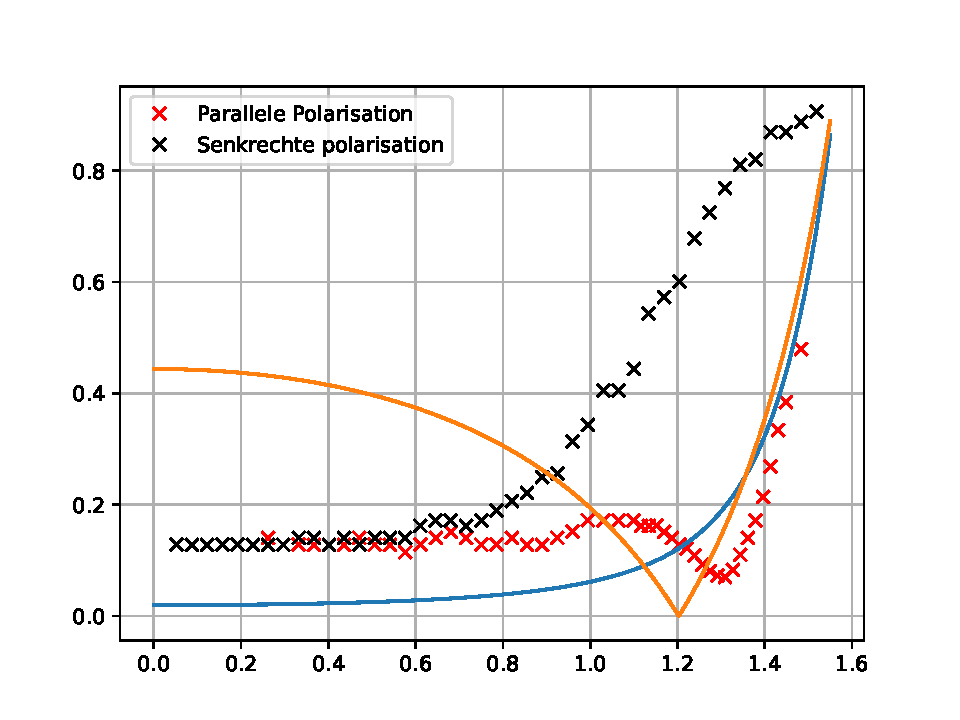
\includegraphics{"build/plot.pdf"}
\end{figure}
\noindent Die Messwerte für $\frac{U_{Br}}{U_s}\left(\Omega\right)$ sind in
\autoref{fig:ub} zusammen mit einer Theoriefunktion, bestimmt aus
\autoref{eqn:omega}, abgebildet.

\noindent Aus diesen Messwerten soll der Klirrfaktor der Speisespannung ermittelt werden. 
Dies geschieht durch das Ermitteln der Restspannung $U_\text{Rest}$. Diese 
Restspannung wird mit dem Koeffizienten $g(2)$ multipliziert, welcher dem 
Verhältnis $\frac{U_\text{Br}}{U_\text{s}}$ aus \autoref{eqn:1} bei $\Omega = 2$ entspricht, um so 
einen Wert für die Amplitude der zweiten Oberwelle $U_2$ zu erhalten.
Daraus lässt sich durch \autoref{eqn:Klirrfaktor} der Klirrfaktor berechnen,
wenn die Annahme getroffen wird, dass nur die zweite Oberwelle wesentlich zum
Klirrfaktor beiträgt. Des Weiteren wird angenommen, dass der Klirrfaktor klein
ist. Es wird  $U_1 = U_\text{s}$ genähert.
Die Restspannung bei $\Omega = 0 $ entspricht 
\begin{equation*}
       U_\text{rest} = 240 \unit{\volt},
\end{equation*}
was zu einem Klirrfaktor von 
\begin{equation*}
       k = \frac{U_2}{U_1} = \frac{U_\text{rest} \cdot \frac{U_\text{Br}}{U_\text{s}}(\Omega = 2)}{U_\text{s}} = \qty{0.0357}{}
\end{equation*}
führt.